\chapter{Diseño\label{sec:diseño}}

Este proyecto \cite{Cano} consiste en una ampliación y cambio de enfoque de otro proyecto llevado a cabo de manera simultánea por una alumna de la Universidad Politécnica de Madrid llamada Nerea Urrestarazu que a su vez se basa en el Kit de demostración de rendimiento del ADS1299 proporcionado por Texas Instrument.

\begin{figure} [h]
    \centering
    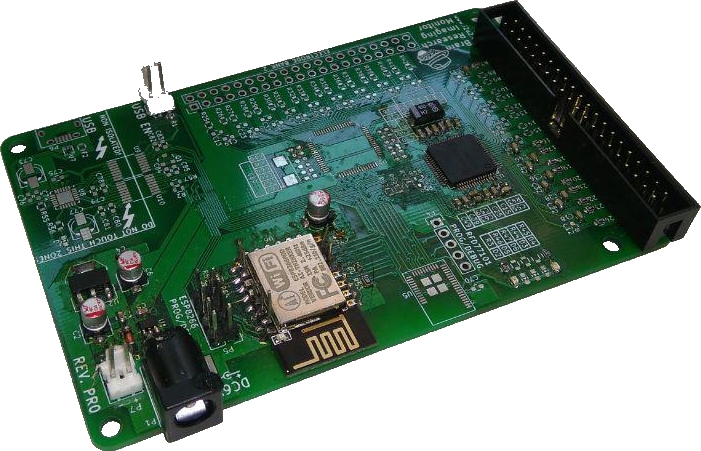
\includegraphics[width=7cm]{Placa_Nerea}
    \caption{Placa final del proyecto base}
    \label{fig:Placa_base}
\end{figure}

\section{Diseño base\label{sec:Diseno_base_N}}

El proyecto original trata sobre el diseño y desarrollo de una placa de adquisición de EEG haciendo uso de los integrados ADS1299 junto con un sistema de transmisión hacia el ordenador tanto inalámbricamente como a través de USB. La figura \ref{fig:Diseno_base} muestra las partes que componen dicho diseño.

\begin{figure} [h]
    \centering
    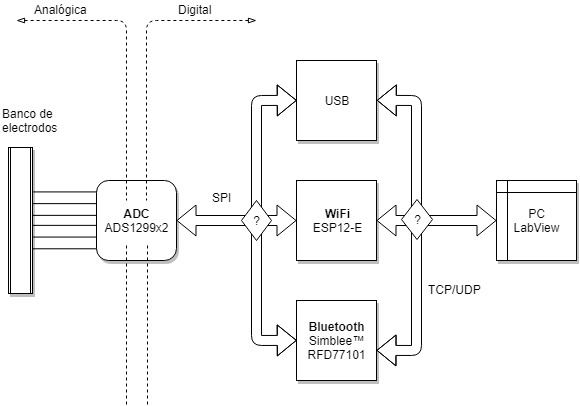
\includegraphics[width=12cm]{Esquema_diseno_base}
    \caption{Esquema del proyecto base}
    \label{fig:Diseno_base}
\end{figure}

\section{Adquisición de datos\label{sec:Adquisicion_N}}

La parte encargada de la adquisición está compuesta por un par de bancos de electrodos dispuestos en los laterales de la placa seguidos de un filtro paso-bajo con frecuencia de corte de 6.79kHz encargado de eliminar las componentes de frecuencias muy altas, no deseadas en el estudio de un \acrshort{EEG}. A continuación se encuentran conectados a sus respectivos bancos los \acrshort{ADC} ADS1299. 
\\Estos convertidores son capaces de adquirir información de forma independiente o en modo ``Daisy Chain'' y transmitirla a través de \acrshort{SPI} hacia otros dispositivos cuya misión será gestionarla.

\begin{figure} [h]
    \centering
    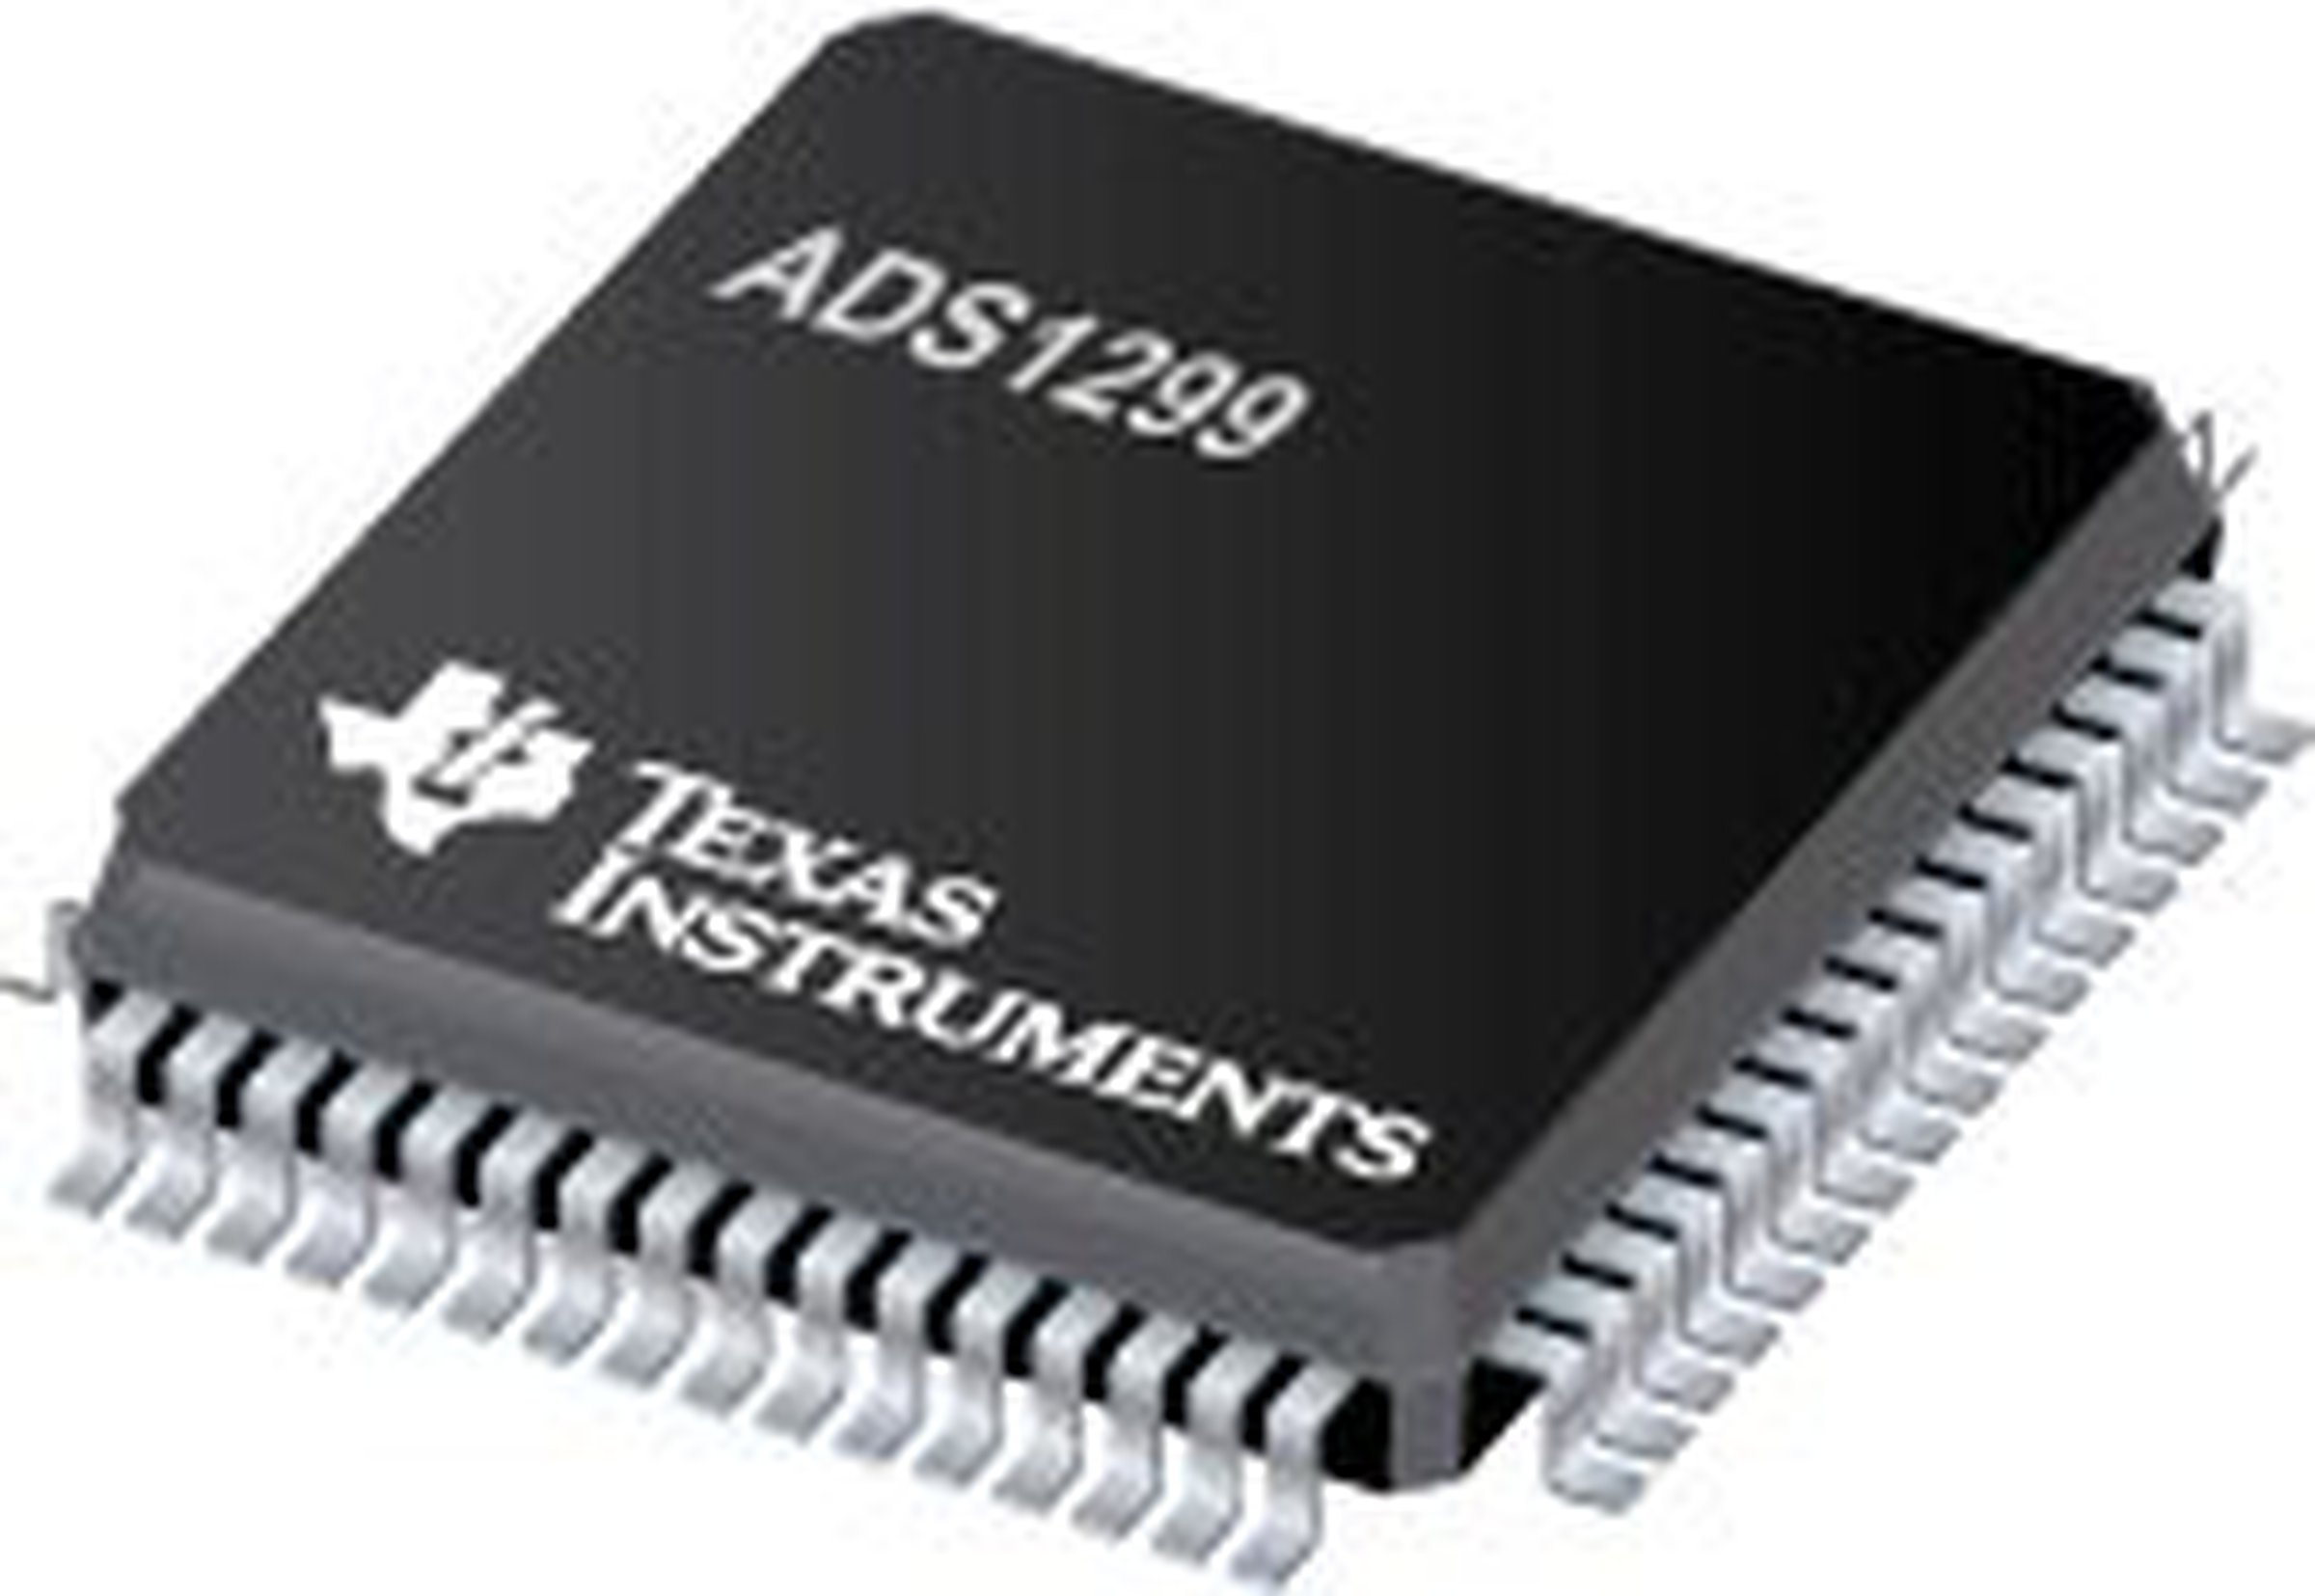
\includegraphics[width=7cm]{ADS1299}
    \caption{Convertidor Analógico-Digital ADS1299}
    \label{fig:ADS1299}
\end{figure}

El \acrshort{SPI} presente en el convertidor permite leer todos los registros del ADS y escribir la gran mayoría. Aunque normalmente se leen los relacionados con los datos convertidos, también es posible saber el estado de los \acrshort{GPIO} o el identificador único del dispositivo leyendo su registro asociado.

La configuración del ADS se realiza mediante la escritura de ciertos registros, cada uno asociado a un parámetro específico. La tabla \ref{tab:Conf_Reg_ADS} muestra los registros disponibles, tanto de lectura como de configuración, una descripción básica y la dirección de memoria asociada a los mismos.

\begin{table} [h]
    \centering
    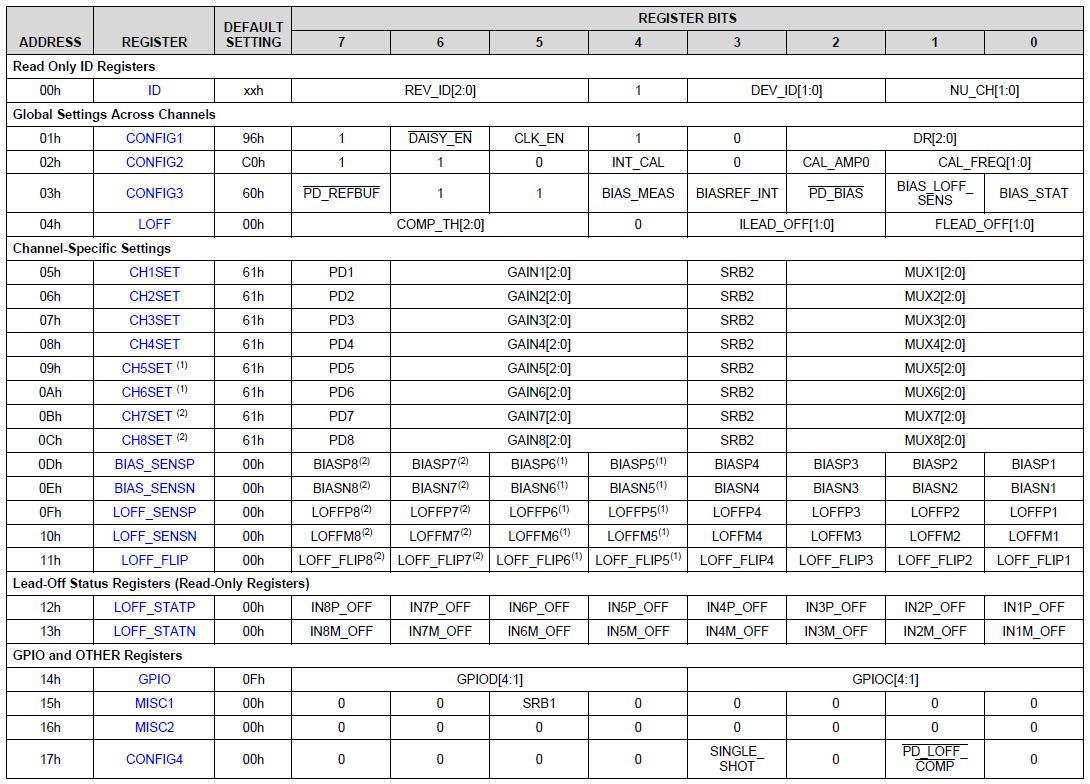
\includegraphics[width=\textwidth]{Tabla_registros_ADS}
    \caption{Tabla de registros de la familia ADS}
    \label{tab:Conf_Reg_ADS}
\end{table}

Una descripción más detallada de cada uno de los bits de cada registro se puede encontrar en el \textit{datasheet} del componente.

Como se puede ver en la tabla \ref{tab:Conf_Reg_ADS}, los convertidores cuentan con una gran cantidad de opciones de configuración. Para el desarrollo de este proyecto se ha implementado un sistema de configuración que permite cambiar el valor de todos los registros.

\section{Transmisión de datos\label{sec:Transmisión_N}}

Una vez se ha capturado y convertido la información es necesario transmitirla, para ello la placa original contaba con dos alternativas. La primera consiste en, mediante \acrshort{USB} y acopladores aislantes, transmitir la información a un ordenador. 
\\La segunda hace uso de dos tecnologías inalámbricas distintas que funcionan de forma excluyente, seleccionables con un \textit{jumper}: WiFi o Bluetooth.

\subsection{WiFi\label{sec:WiFi_N}}

Para la transmisión de datos a través de WiFi se seleccionó el módulo ESP12-E, basado en el \acrshort{SoC} ESP2866, también conocido nodemcu.
\\Este cuenta con un microcontrolador embebido de 32 bits (Tensilica L106) con una memoria \acrshort{RAM} de 36kB y una velocidad de reloj de la \acrshort{CPU} de hasta 80MHz, proporcionando suficiente potencia para las tareas básicas.

Así mismo se incluye montado en el mismo paquete una memoria flash de 4MB en la que almacenar el código de los programas que se ejecutarán. 

\begin{figure} [h]
    \centering
    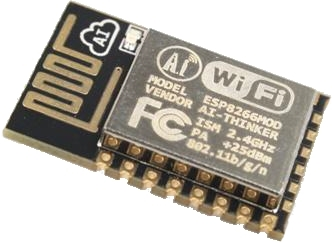
\includegraphics[width=7cm]{ESP8266}
    \caption{ESP8266}
    \label{fig:ESP8266}
\end{figure}

A efectos de diseño es muy importante saber cuales serán las entradas/salidas del dispositivo así como los pines dedicados para su programación. La figura \ref{fig:ESP8266_pinout} muestra un resumen de todas las funciones de cada uno de los pines. Como se puede observar, el \acrshort{SPI} hace uso de los pines 5, 6, 7 y 16. Por otro lado el \acrshort{UART}, necesario para la programación del micro hace uso de los pines 16 y 17. Dichos pines deberán reservarse posteriormente en la fase de diseño de la \acrshort{PCB}.

\begin{figure} [h]
    \centering
    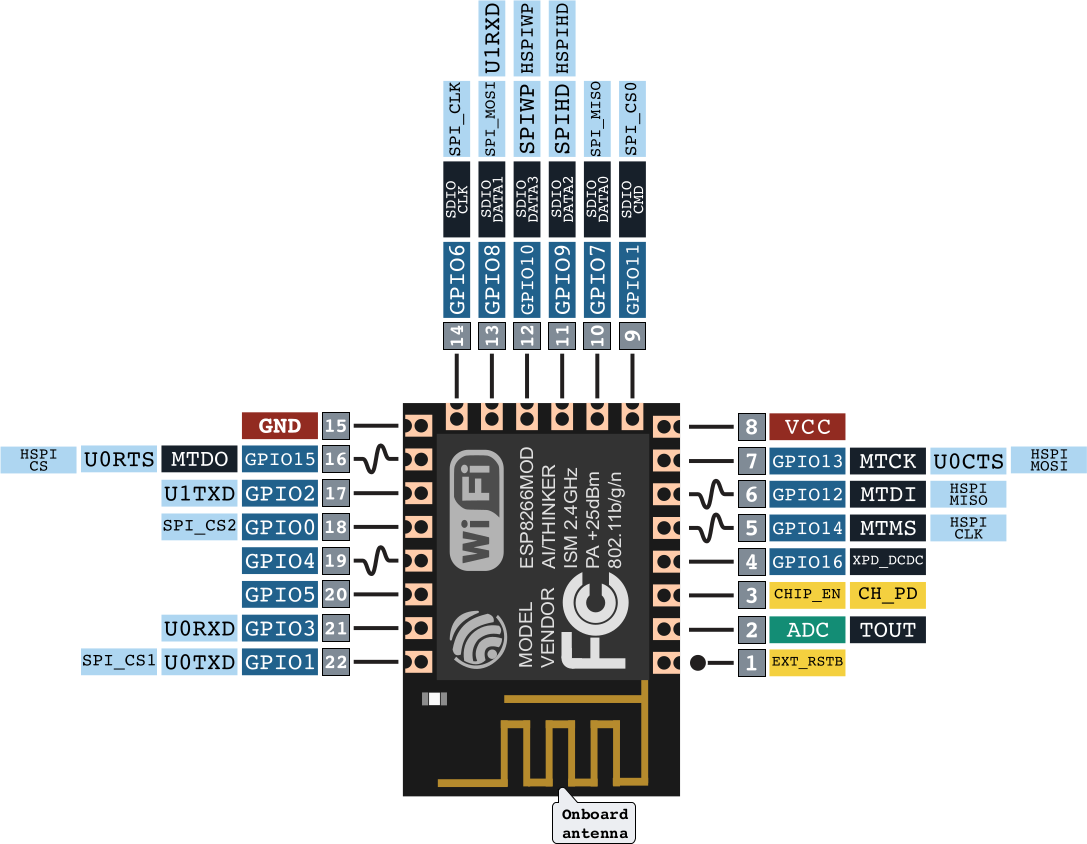
\includegraphics[width=\textwidth]{esp8266-esp12e-pinout}
    \caption{Resumen de todas las Entradas/Salidas del ESP12-E}
    \label{fig:ESP8266_pinout}
\end{figure}

El dispositivo tiene tres modos de arranque dependiendo del sitio desde el que cargue el código y la selección de uno u otro modo viene determinada por los pines MTDO, GPIO0 y GPIO2. \\La tabla \ref{tab:ESP_Boot_Modes} resume los distintos modos de arranque así como el estado en el que debe estar cada uno de los pines para entrar en ese modo.
\begin{table} [h]
 	\centering
	\begin{tabular}{|c|c|c|c|c|}
		\hline 
		MTDO & GPIO0 & GPIO2 & Modo & Descripción \\ 
		\hline 
		L & L & H & UART & Descarga el código desde UART \\ 
		\hline 
		L & H & H & Flash & Carga desde memoria Flash a través de SPI \\ 
		\hline 
		H & x & x & SDIO & Carga desde una tarjeta SD \\ 
		\hline 
	\end{tabular} 
	\caption{Modos de arranque del ESP12-E}
    \label{tab:ESP_Boot_Modes}
\end{table}	

\subsection{Bluetooth\label{sec:Bluetooth_N}}



\subsection{USB\label{sec:USB_N}}


Como este proyecto tiene como objetivo independizar el sistema lo máximo posible del ordenador se ha optado por desestimar el sistema de transmisión por \acrshort{USB} conservando solamente la interfaz inalámbrica. 

Hablar de la placa de Nerea y cómo la haces inteligente

Selección del STM

Diseño de la placa

	Comunicación con la otra placa (sandwich) vs Diseño de cero
	Alimentación
	Interfaces
